\section{Технический проект}
\subsection{Общие сведения о программной системе}

Необходимо спроектировать и реализовать веб-приложение, которое будет предназначено для освещения инцидентов, связанных с общественным транспортом, таких как автобусы, троллейбусы и маршрутные такси. В веб-приложение предоставит пользователям возможность просматривать посты и видеозаписи, содержащие информацию об инцидентах с общественным транспортом. 

Для доступа к просмотру или оставлению обращений пользователи должны будут зарегистрироваться или войти в систему, что обеспечит контроль над контентом и позволит отслеживать активность каждого пользователя. Пользователи смогут оставлять свои обращения о случившихся инцидентах, заполняя форму обратной связи, где они будут описывать произошедшее событие. Зарегистрированные пользователи смогут просматривать все доступные посты и видеозаписи, связанные с инцидентами, которые будут отображаться в формате новостной ленты. Все оставленные обращения будут проходить обязательную модерацию, где тексты проверяются на отсутствие неподобающего контента. Только обращения, прошедшие модерацию, будут публиковаться в ленте.

Администраторы получат расширенные права доступа, позволяющие им добавлять новых водителей в базу данных, редактировать существующую информацию, а также управлять обращениями. Административная панель предоставит все необходимые инструменты для этих задач. В приложении будет предусмотрена функция отображения рейтинга водителей, что позволит пассажирам оценивать их работу и оставлять обратную связь. Пользователи также будут иметь доступ к личному кабинету, где они смогут управлять своей информацией, просматривать свои обращения и взаимодействовать с приложением. Это веб-приложение будет реализовано для освещения инцидентов, связанных с общественным городским транспортом, и будет служить платформой для обмена информацией между пассажирами и ответственными органами. 

Основная цель системы — предоставлять актуальные данные о происшествиях, чтобы ответственные службы могли оперативно реагировать на возникающие проблемы и улучшать качество обслуживания общественного транспорта.

\subsection{Проектирование архитектуры программной системы}

\subsubsection{Выбор архитектурного стиля и паттернов проектирования}

Архитектурный стиль и паттерны проектирования играют важную роль в создании высокопроизводительных, масштабируемых и безопасных систем, особенно когда речь идет о разработке REST API. REST API, или Representational State Transfer Application Programming Interface, представляет собой архитектурный стиль, который опирается на принципы унификации интерфейсов и передачи состояния между клиентом и сервером. При разработке REST API чрезвычайно важно правильно выбрать архитектурный стиль и использовать соответствующие паттерны проектирования, чтобы обеспечить эффективную работу системы и удовлетворить потребности пользователей.

Один из ключевых паттернов проектирования, который можно использовать при разработке REST API, - это паттерн Facade. Паттерн Facade позволяет создать унифицированный интерфейс для взаимодействия с комплексной системой, скрывая детали реализации и предоставляя простой и понятный интерфейс для внешних клиентов. Применение этого паттерна позволяет сделать REST API более модульным и гибким, упрощая его использование и поддержку.

Еще один важный паттерн - это Адаптер. В контексте REST API, Адаптер позволяет преобразовывать данные из одного формата в другой, обеспечивая совместимость между различными системами и источниками данных. Например, если данные получаются в формате, который необходимо преобразовать для работы с REST API, Адаптер может быть использован для выполнения этой задачи, обеспечивая единый формат данных для всей системы.

Клиент-серверная архитектура также играет важную роль в разработке REST API. Этот архитектурный стиль разделяет систему на две основные части: клиентскую сторону, которая отправляет запросы на сервер, и серверную сторону, которая обрабатывает эти запросы и возвращает результаты. Это позволяет создать масштабируемую и гибкую систему, которая может обрабатывать большие объемы запросов от множества клиентов одновременно.

Для обеспечения безопасности данных в REST API широко используются протокол HTTPS и технология ODBC (Open Database Connectivity). HTTPS обеспечивает защищенное соединение между клиентом и сервером, шифруя данные и предотвращая их несанкционированный доступ или изменение. ODBC, с другой стороны, предоставляет универсальный интерфейс для доступа к различным базам данных, позволяя безопасно и эффективно работать с данными в REST API.

Архитектура всей системы представлена на рисунке ~\ref{templ:image2}.
\begin{figure}[H]
	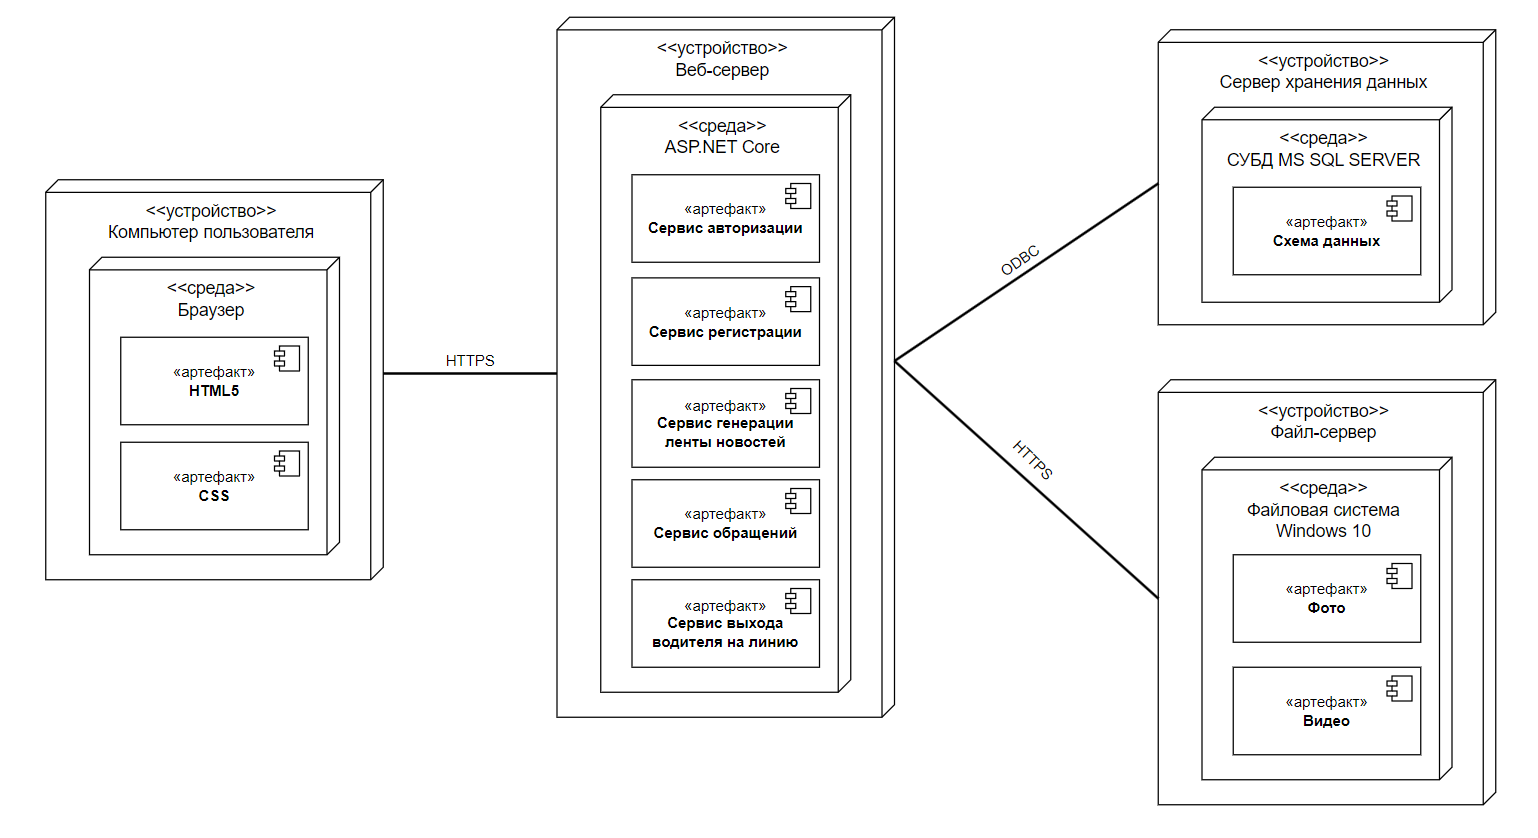
\includegraphics[width=1\linewidth]{Архитектура программной системы}
	\caption{Архитектура программной системы}
	\label{templ:image2}
\end{figure}

\subsubsection{Структура базы данных}

В качестве системы управления базами данных была выбрана реляционная СУБД Microsoft SQL Server. Она предназначена для хранения и управления данными, а также для выполнения различных задач по их обработке, анализу и управлению. SQL Server используется в корпоративных приложениях, веб-приложениях и других системах, где требуется надежное и масштабируемое хранилище данных.

Microsoft SQL Server обладает рядом преимуществ, которые делают его оптимальным выбором для управления базами данных в различных проектах. К ключевым преимуществам можно отнести:
\begin{itemize}
	\item Высокая производительность. SQL Server оптимизирован для высокой производительности как для транзакционных рабочих нагрузок, так и для аналитических запросов. Он включает в себя технологии, такие как in-memory processing и параллельное выполнение запросов, что позволяет обрабатывать большие объемы данных эффективно.
	\item Безопасность данных. SQL Server предоставляет обширные возможности для обеспечения безопасности данных. В него встроены функции шифрования данных, аутентификации, управления доступом на основе ролей (RBAC), а также средства для аудита и мониторинга безопасности.
	\item Высокая доступность и отказоустойчивость. Существует несколько функций для обеспечения высокой доступности и отказоустойчивости, включая Always On Availability Groups, репликацию и зеркалирование баз данных. Эти функции помогают минимизировать время простоя и обеспечивают непрерывный доступ к данным.
	\item Масштабируемость. SQL Server может масштабироваться как вертикально, так и горизонтально. Он поддерживает работу на разных уровнях — от небольших приложений до крупных корпоративных систем с большими объемами данных и высокой нагрузкой.
	\item Обширная поддержка и документация. Microsoft предоставляет обширную документацию, поддержку и ресурсы для обучения. Это включает в себя онлайн-документацию, форумы, обучающие курсы и официальные сертификации, что помогает администраторам и разработчикам быстро освоить и эффективно использовать SQL Server.
\end{itemize}

Несмотря на многочисленные преимущества, Microsoft SQL Server имеет и некоторые недостатки, которые могут быть значимыми в зависимости от конкретных требований и условий эксплуатации. К недостаткам можно отнести:
\begin{itemize}
	\item Обновления и совместимость. Обновления SQL Server могут вызывать затруднения и иногда могут создавать проблемы с совместимостью приложений, особенно если они зависят от определенных версий или функций базы данных. Это требует тщательного планирования и тестирования перед внедрением обновлений.
	\item Ограниченная кроссплатформенность. Хотя в последние годы Microsoft сделала шаги в сторону кроссплатформенности (например, выпустила версии SQL Server для Linux), основная платформа и многие функции SQL Server всё ещё оптимизированы для работы на Windows. 
	\item Требования к аппаратному обеспечению. Для достижения максимальной производительности SQL Server требует значительных ресурсов аппаратного обеспечения, таких как процессор, память и дисковое пространство.
\end{itemize}

На основании анализа предметной области и технического задания была разработана база данных, предназначенная для хранения и обработки хранящейся информации. Схема данных представлена на рисунке ~\ref{templ:image1}.
\begin{figure}[H]
	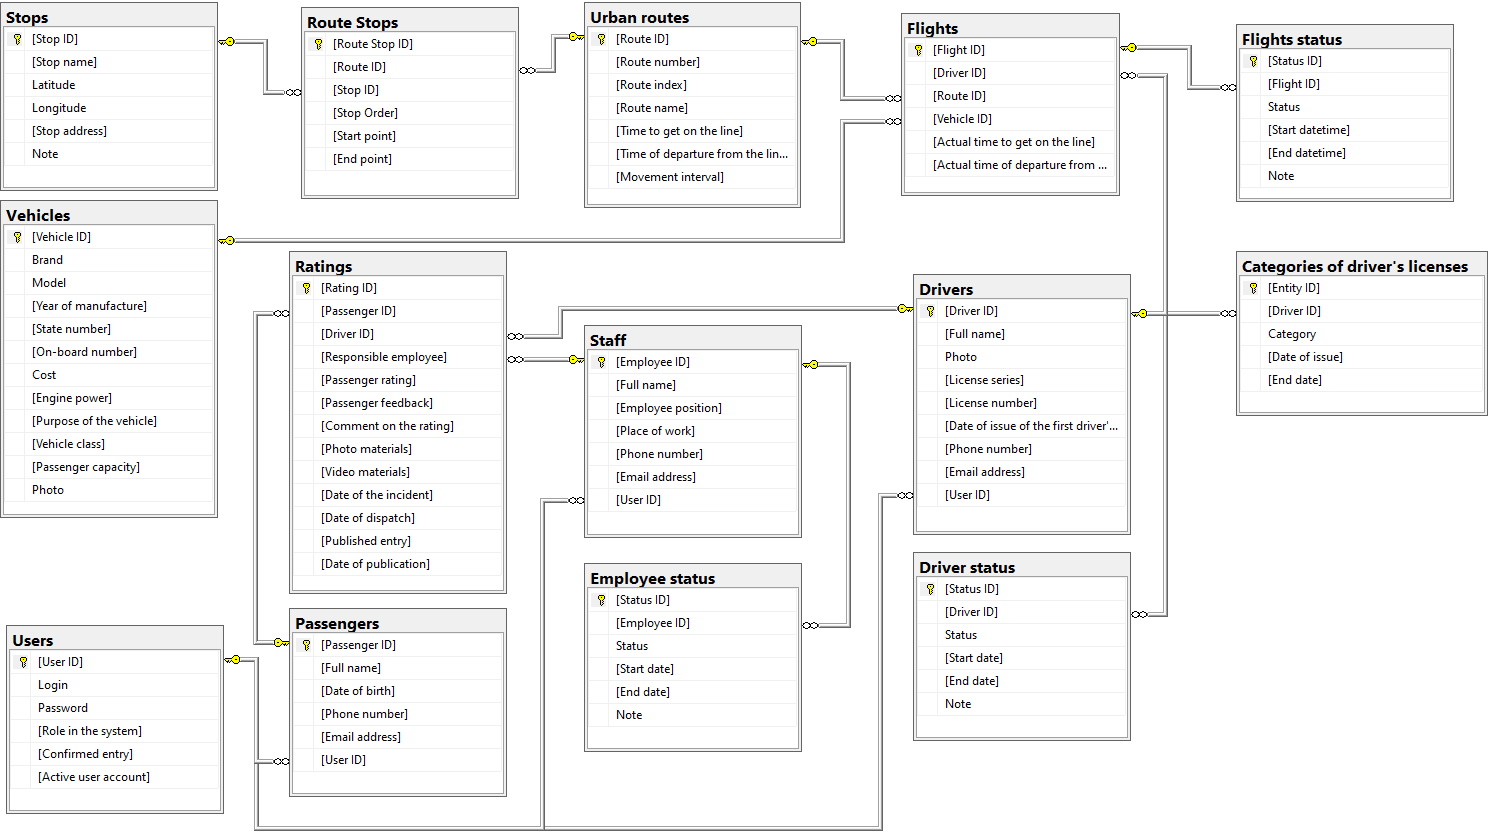
\includegraphics[width=1\linewidth]{Схема данных}
	\caption{Схема данных}
	\label{templ:image1}
\end{figure}

Все сущности базы данных приведены к третьей нормальной форме, что означает, что каждая таблица удовлетворяет требованиям нормализации:
\begin{enumerate}
	\item Отсутствие дублирования данных. В каждой таблице данные не дублируются, что помогает избежать избыточности и обеспечивает экономное использование ресурсов.
	\item Зависимость атрибутов от первичного ключа. Все неключевые атрибуты в таблице зависят только от первичного ключа, а не от других неключевых атрибутов. Это гарантирует, что каждая таблица содержит данные, относящиеся к одному логическому объекту или концепции.
	\item Устранение транзитивных зависимостей. Если атрибуты зависят друг от друга через другой атрибут, такие зависимости устранены. Это обеспечивает целостность данных и упрощает процесс обновления и удаления данных.
\end{enumerate}

Приведение базы данных к третьей нормальной форме помогает повысить эффективность запросов, уменьшить риск возникновения аномалий при обновлении данных и повысить отказоустойчивость.

\subsubsection{Описание микросервисов}
Микросервисы играют ключевую роль в разрабатываемом веб-приложении, поскольку они обеспечивают модульную архитектуру, гибкость и масштабируемость системы. Каждый микросервис представляет собой отдельную функциональную единицу, специализирующуюся на определенной задаче, что позволяет легко разрабатывать, развертывать и масштабировать приложение.
\begin{enumerate}
	\item Микросервис обработки обращений
	
	Назначение: Обработка обращений от граждан, связанных с инцидентами на общественном транспорте.
	
	Функции: Прием обращений, проверка корректности данных, направление обращений на модерацию администратору.
	
	Преимущества: Обеспечивает структурированное и оперативное управление обращениями, что способствует быстрому реагированию на проблемы и улучшению качества обслуживания пассажиров.
	
	\item Микросервис аутентификации и авторизации пользователей
	
	Назначение: Обеспечение безопасного доступа пользователей к веб-приложению.
	
	Функции: Управление регистрацией новых пользователей, проверка учетных данных при входе, назначение ролей и прав доступа.
	
	Преимущества: Гарантирует, что только авторизованные пользователи могут оставлять обращения и получать доступ к персонализированным функциям приложения, обеспечивая безопасность данных и предотвращение несанкционированного доступа.
	
	\item Микросервис работы с базой данных через панель администратора (управление базой данных)
	
	Назначение: Управление базой данных администратором системы.
	
	Функции: Добавление новых водителей в базу данных, редактирование и удаление информации, мониторинг активности пользователей, управление обращениями и отчетами.
	
	Преимущества: Обеспечивает администратору удобные инструменты для управления данными, что повышает эффективность администрирования и поддержания актуальности данных.
	
	\item Микросервис регистрации
	
	Назначение: Обеспечение удобного процесса регистрации новых пользователей в системе.
	
	Функции: Обработка регистрационных данных, проверка уникальности пользователей, отправка подтверждений по электронной почте.
	
	Преимущества: Облегчает процесс регистрации, повышая удобство для пользователей и увеличивая количество участников, активно использующих приложение.
\end{enumerate}

Эти микросервисы интегрированы для создания эффективной и надежной системы управления инцидентами в общественном транспорте. Они обеспечивают структурированный подход к обработке обращений, защиту данных, гибкость управления и удобство для конечных пользователей, что в конечном итоге способствует улучшению качества обслуживания и повышению доверия к транспортным службам.

\subsection{Обоснование выбора технологии проектирования}

В настоящее время информационный рынок, предоставляющий программные решения в выбранной сфере, предлагает множество продуктов, которые позволяют успешно разработать веб-приложение и достигнуть поставленной цели.

\subsubsection{Описание используемых технологий и языков программирования}

В процессе разработки веб-приложения используются различные программные средства и языки программирования, каждый из которых применяется для выполнения специфических задач, необходимых для реализации проекта.

\subsubsection{Язык программирования JavaScript}

Выбор языка программирования JavaScript для разработки микросервисов также обосновывается несколькими ключевыми преимуществами этого языка. Прежде всего, JavaScript является одним из самых популярных языков программирования, широко используемым в веб-разработке. Его широкое распространение обусловлено его универсальностью и возможностью использования как на стороне клиента (браузер), так и на стороне сервера (Node.js).

Второе важное преимущество JavaScript - его высокая гибкость и динамичность. JavaScript позволяет быстро создавать интерактивные и динамические пользовательские интерфейсы, что особенно важно для микросервисов, предоставляющих данные веб-приложениям.

Третье преимущество JavaScript - его асинхронная природа. JavaScript поддерживает асинхронное программирование, что позволяет эффективно обрабатывать большие объемы запросов и взаимодействовать с базами данных и другими внешними ресурсами без блокировки выполнения программы.

Наконец, JavaScript обладает обширной экосистемой библиотек и фреймворков, таких как Express.js для серверной разработки, React.js и Vue.js для разработки пользовательских интерфейсов, что делает его привлекательным выбором для создания микросервисных архитектур.

В целом, JavaScript представляет собой мощный инструмент для разработки микросервисов, обеспечивая высокую гибкость, производительность и возможность масштабирования системы.

\subsubsection{Язык программирования C\#}

Выбор языка программирования C\# для разработки микросервисов обусловлен несколькими ключевыми преимуществами этого языка. Прежде всего, C\# известен своей высокой производительностью, что обеспечивает быстрое выполнение программы. Второе важное преимущество - масштабируемость. С помощью C\# легко создавать системы, способные масштабироваться в соответствии с растущими потребностями. И наконец, кросс-платформенность делает C\# универсальным языком программирования, что позволяет разрабатывать приложения, работающие на различных операционных системах. Все эти факторы совместно обеспечивают быструю разработку надежной и масштабируемой системы при использовании C\#.

\subsubsection{HTML}

HTML является стандартным языком разметки, широко используемым для создания структуры веб-страниц. Выбор HTML для разработки микросервисов также имеет свои преимущества.

Во-первых, HTML является основным строительным блоком веб-страниц и обеспечивает их структуру и семантику. Это позволяет легко создавать пользовательские интерфейсы и представления для микросервисов, делая их интуитивно понятными и удобными для пользователей.

Во-вторых, HTML легко интегрируется с другими технологиями веб-разработки, такими как CSS для стилизации и JavaScript для создания интерактивных элементов. Это позволяет создавать более сложные и функциональные веб-приложения на основе микросервисной архитектуры.

Третье преимущество HTML - его доступность и поддержка во всех современных браузерах. Это обеспечивает широкий охват аудитории и упрощает развертывание и поддержку веб-приложений на основе микросервисов.

Наконец, HTML обладает простым и интуитивно понятным синтаксисом, что делает его доступным даже для новичков в веб-разработке. Это упрощает процесс создания и поддержки микросервисов, особенно при работе в команде.

В целом, HTML является важным инструментом для создания пользовательских интерфейсов и представлений в микросервисной архитектуре. Его простота, доступность и гибкость делают его привлекательным выбором для разработки веб-приложений любого уровня сложности.

\subsubsection{React}

React - это JavaScript-библиотека, разработанная для создания пользовательских интерфейсов веб-приложений. Выбор React для разработки микросервисов также имеет свои преимущества.

Во-первых, React предоставляет удобный и эффективный способ создания динамических пользовательских интерфейсов. Он использует компонентный подход, позволяя разбивать пользовательский интерфейс на множество небольших и переиспользуемых компонентов. Это делает код более чистым, модульным и легко поддерживаемым.

Во-вторых, React обеспечивает высокую производительность благодаря виртуальному DOM. Виртуальный DOM позволяет React оптимизировать обновление пользовательского интерфейса, перерисовывая только те компоненты, которые действительно изменились. Это делает React идеальным выбором для создания микросервисов с высокой производительностью и быстрой отрисовкой.

Третье преимущество React - его обширная экосистема. Существует множество дополнительных библиотек и инструментов, таких как Redux для управления состоянием, React Router для навигации в приложении, и многие другие, которые облегчают разработку микросервисов на основе React.

 React представляет собой мощный инструмент для разработки микросервисов, обеспечивая высокую производительность, модульность и широкие возможности для создания динамичных пользовательских интерфейсов.